\documentclass[12pt]{article}
\usepackage[utf8]{inputenc}
\usepackage{graphicx}
\usepackage{amsmath,amsfonts,amssymb}
\usepackage{algorithm}
\usepackage{algpseudocode}
\usepackage{geometry}
\usepackage{url}
\usepackage{hyperref}
\usepackage{enumitem}
\usepackage{caption}
\usepackage{float}
\usepackage[most]{tcolorbox}
\geometry{margin=1in}
\tcbuselibrary{listingsutf8}


\title{}
\author{Yuguang YAO and Duc Khoi LE  \textit{\small Ecole Polytechnique}}
\date{May 2025}

\begin{document}

\maketitle

\begin{abstract}
This project focuses on the analysis of scientific papers in the field of high-energy theoretical physics, based on metadata and abstracts from the hep-th (High Energy Physics - Theory) category on arXiv. The dataset spans papers submitted between 1992 and 2003. The main objectives are:
\begin{itemize}
\item To analyze the evolution of research topics and trends within the field;
\item To build a semantic graph of papers using natural language processing techniques (e.g., keyword extraction and sentence embeddings);
\item To apply graph theory algorithms to identify key papers, domain clusters, and citation flows;
\item To visualize the results interactively, offering researchers an intuitive understanding of the field’s structure.
\end{itemize}
The document covers dataset description, preprocessing steps, keyword extraction methods (such as BertKey), graph construction and clustering algorithms (e.g., HDBSCAN), and visualization tools (such as ipysigma). It also includes illustrative figures and technical implementation details.
\end{abstract}

\tableofcontents

\newpage

\section{Introduction}

Scientific collaboration has become increasingly data-rich, with large-scale metadata repositories like arXiv offering valuable insights into the dynamics of academic production. This project seeks to investigate the structure of high-energy theoretical physics through the lens of co-authorship, citation, and keyword-based clustering. We analyze papers submitted between 1992 and 2003 in the \texttt{hep-th} category on arXiv, using graph-theoretic and NLP-based methods.

While the objectives are ambitious and the methodological diversity is commendable, several foundational aspects of the project warrant critical scrutiny. First, the document lacks a clear articulation of the central research question. It proceeds with multiple computational steps—graph construction, clustering, citation trees—without clarifying what specific patterns or hypotheses are being tested. This risks turning the work into a purely descriptive effort, rather than a scientifically driven inquiry.

Second, although the dataset spans more than a decade, there is limited reflection on the limitations or biases inherent in the corpus (e.g., language uniformity, geographic skew, or disciplinary overlap with adjacent subfields). Moreover, while advanced tools such as BERT-based keyword extraction and Louvain community detection are employed, the project would benefit from a justification of why these specific techniques were chosen over alternatives. For instance, no performance evaluation or comparative benchmark is given for the keyword extraction method.

Finally, the introduction makes no mention of how the results are intended to inform or benefit the broader research community. What concrete insight is expected for physicists, historians of science, or bibliometricians? Without such context, the work risks being technically impressive but epistemically opaque.

In this report, we attempt to address these gaps where possible, and structure our analysis across data description, graph construction, community detection, semantic clustering, and citation flow modeling. Throughout, we adopt a critical perspective, evaluating not only the results but also the assumptions, limitations, and future directions that accompany each stage.


\section{Dataset Description and Motivation}

\subsection{Overview of the Dataset}

The dataset used in this project consists of metadata and abstracts from scientific papers in the field of high-energy theoretical physics, specifically from the \texttt{hep-th} (High Energy Physics - Theory) category on arXiv. The data spans papers submitted between the years \textbf{1992 and 2003}, providing over a decade of publication activity. Instead of using data mining, we download the data from Stanford Large Network Dataset Collection. We use two data bases: High Energy Physics - Theory collaboration network and High-energy physics theory citation network.

An example is shown below:

\begin{tcolorbox}
------------------------------------------------------------------------------

\textbackslash\textbackslash{}

Paper: hep-th/9201001

From: zuber@poseidon.saclay.cea.fr (C. Itzykson)

Date: Tue Dec 31 23:54:17 MET 1991 +0100   (37kb)

Title: Combinatorics of the Modular Group II: the Kontsevich integrals

Authors: C. Itzykson and J.-B. Zuber

Comments: 46 pages

Subj-class: High Energy Physics - Theory; Quantum Algebra

Journal-ref: Int.J.Mod.Phys. A7 (1992) 5661-5705

\textbackslash\textbackslash{}

We study algebraic aspects of Kontsevich integrals as generating functions for intersection theory over moduli space and review the derivation of Virasoro and KdV constraints.
1. Intersection numbers
2. The Kontsevich integral
2.1. The main theorem
2.2 Expansion of Z on characters and Schur functions
2.3 Proof of the first part of the Theorem
3. From Grassmannians to KdV
4. Matrix Airy equation and Virasoro highest weight conditions
5. Genus expansion
6. Singular behaviour and Painlev'e equation.
7. Generalization to higher degree potentials
 
\textbackslash\textbackslash{}
\end{tcolorbox}


\subsection{The first extractiong from data}

Specifically, we used the \texttt{cit-HepTh-abstracts} portion of the collection. The files are organized in directories by year --- for example, \texttt{1992/}, \texttt{1993/}, up to \texttt{2003/}. Each directory contains multiple \texttt{.abs} files, one per paper.

To extract relevant information, we developed a Python script called First\_extraction.py to convert the raw text file to .json that iterates through these yearly folders and parses the content of each file. This processing pipeline is detailed in the following section.

\subsection{Motivation for Choosing This Dataset}

We chose this dataset for several reasons:
\begin{itemize}
    \item \textbf{Well-defined collaboration structure:} Research in high-energy theoretical physics often involves co-authorship, making this dataset ideal for network analysis.
    \item \textbf{Temporal richness:} The inclusion of submission dates enables dynamic studies on the evolution of collaboration networks and research topics over time.
    \item \textbf{Scientific significance:} arXiv’s \texttt{hep-th} category is a foundational area of physics with strong academic and citation dynamics.
    \item \textbf{Clean and structured format:} The \texttt{.abs} format facilitates straightforward parsing and metadata extraction for large-scale analysis.
\end{itemize}


\section{Extraction of Paper Metadata and Abstracts}

To initiate our analysis, we begin by collecting and standardizing paper metadata and abstracts from a raw corpus of \texttt{.abs} files. These files are organized by year (from 1992 to 2003) and contain structured header information followed by an abstract. With few test we can run through all fields in the raw file and convert it into \texttt{output.json}.

Python script (\texttt{First\_Extraction.py}) systematically processes each \texttt{.abs} file to extract relevant information. The workflow is as follows:

\begin{enumerate}
    \item \textbf{Preprocessing:} The script removes the first two and the last lines, which often serve as separators. Then it splits the file into a header section and an abstract section using double backslash \texttt{\textbackslash\textbackslash} markers.

    \item \textbf{Header Parsing:} Regular expressions are used to detect known field names (e.g., \texttt{Title:}, \texttt{Authors:}) and map them to standard keys. The parser also supports multiline fields and flags unknown lines for manual review.

    \item \textbf{Abstract Normalization:} The abstract content is cleaned of excess whitespace and concatenated into a single string for uniform processing.

    \item \textbf{Year Derivation:} A year is extracted from the \texttt{submitted} field using regex, with logic to resolve ambiguous formats (e.g., \texttt{02} $\rightarrow$ 2002).
\end{enumerate}

\begin{algorithmic}[1]
    \For{$year$ in $start$ to $end$}
        \For{each \texttt{.abs} file in $year$ directory}
            \State Parse file content $\rightarrow$ structured record
            \State Append record with year to result list
        \EndFor
    \EndFor
    \State Save all records to \texttt{output.json}
\end{algorithmic}

\vspace{1em}

\begin{algorithmic}[1]

    \State Remove header/footer noise
    \State Split into metadata and abstract with slashes
    \For{each line in metadata}
        \If{matches known field}
            \State Store field value
        \Else
            \State Append to last known field
        \EndIf
    \EndFor
    \State Normalize whitespace
    \State Extract year from date if possible
    
    \Return structured data
\end{algorithmic}

\subsection{Data Fields Extracted}


A derived field \texttt{year} was also added derived from \texttt{paper\_id}, parsed from the submission date, to facilitate analysis. An entry from \texttt{output.json} is shown below.

\begin{itemize}
  \item \textbf{paper\_id}: \texttt{hep-th/9207013}
  \item \textbf{from}: \texttt{"Jose M. Figueroa-O'Farrill" <figueroa@pib1.physik.uni-bonn.de>}
  \item \textbf{submitted}: \texttt{Fri, 03 Jul 1992 23:07:20 MEZ (15kb)}
  \item \textbf{title}: \textit{On the two-boson picture of the KP hierarchy}
  \item \textbf{authors}: \texttt{J.M. Figueroa-O'Farrill, J. Mas, and E. Ramos}
  \item \textbf{comments}: \texttt{8 pages, Plain TeX, BONN-HE-92-17, KUL-TF-92/26, US-FT-4/92}
  \item \textbf{report\_no}: \texttt{null}
  \item \textbf{journal\_ref}: \texttt{Phys. Lett. B292 (1992) 337-340}
  \item \textbf{subject\_class}: \texttt{null}
  \item \textbf{proxy}: \texttt{null}
  \item \textbf{abstract}: \smallskip

  \begin{quote}
    A two-boson realization of the second hamiltonian structure for the KP hierarchy has recently appeared in the literature. Furthermore, it has been claimed that this is also a realization of the hierarchy itself. This is surprising because it would mean that the dynamics of the KP hierarchy---which in its usual formulation requires an infinite number of fields---can be described with only two. The purpose of this short note is to point out the almost obvious fact that the hierarchy described by the two bosons is not the KP hierarchy but rather a reduction thereof---one which is moreover incompatible with the reduction to the KdV-type subhierarchies.
  \end{quote}

  \item \textbf{year}: \texttt{1992}
\end{itemize}

\subsection{Parsing Method}



\subsection{Batch Processing and Output}

The script processes yearly directories from 1992 to 2003. For each valid \texttt{.abs} file:
\begin{itemize}
    \item A dictionary of extracted fields is created.
    \item All dictionaries are collected into a list and saved as \texttt{output.json} using UTF-8 encoding with pretty formatting.
\end{itemize}






\begin{verbatim}
with open('output.json', 'w', encoding='utf-8') as f:
    json.dump(results, f, ensure_ascii=False, indent=2)
\end{verbatim}

In total, the pipeline processed \texttt{N} records (with the exact count printed at runtime), producing a clean and structured dataset ready for further analysis such as graph construction and author network modeling.

\section{Name Cleaning and Author Name Standardization}

\subsection{Motivation}
From the \texttt{output.json}, we have now a string that encodes the authors that could be:
\begin{tcolorbox}
"authors": "J.M. Figueroa-O'Farrill, E. Ramos, and S. Stanciu"

"authors": "Mark Doyle (Princeton University)"

"authors": "Curtis G. Callan, Jr., Juan M. Maldacena and Amanda W. Peet (Princeton University)"

"authors": "O. Aharony, S.S. Gubser, J. Maldacena, H. Ooguri, and Y. Oz",
\end{tcolorbox}


In the context of analyzing scientific collaboration networks, accurate identification of individual authors is essential. However, inconsistencies in name formatting across submissions can lead to inflated or fragmented author identities. For example, ``J. Maldacena'' and ``Juan Maldacena'' may refer to the same individual but would be treated as distinct nodes in a graph if not normalized. To address this, we designed a two-stage name cleaning pipeline to extract, clean, and standardize author names across the dataset.

\subsection{Stage 1: Name Extraction and Initial Cleaning}

The first stage is implemented in \texttt{nom.py}, which reads the \texttt{authors} field from the \texttt{output.json} file and generates a cleaned list of unique author names.

\begin{itemize}
    \item Author strings are preprocessed by:
        \begin{itemize}
            \item Removing quotation marks and parentheses
            \item Replacing multiple spaces with single spaces
            \item Splitting names based on commas and conjunctions (e.g., ``and'')
            \item Stripping institutional affiliations or emails using keyword heuristics
        \end{itemize}
    \item Names are filtered to exclude entries likely to be institutions, using rules based on:
        \begin{itemize}
            \item Presence of academic keywords (e.g., ``university'', ``institute'')
            \item Email patterns (e.g., containing ``@'')
            \item All-uppercase tokens resembling acronyms
        \end{itemize}
    \item The resulting list of author names is exported to \texttt{authors.csv}, sorted alphabetically.
\end{itemize}

This stage produces a high-quality set of candidate personal names, minimizing noise from affiliations or malformed entries.

\subsection{Stage 2: Standardization via Name Variant Merging}

In the second stage, implemented in \texttt{standarniee\_name.py}, we resolve naming inconsistencies using string normalization, name parsing, and clustering techniques.

\subsubsection*{Parsing and Variant Generation}

\begin{itemize}
    \item Each name is parsed into first names and last name components. Compact forms (e.g., ``JMMaldacena'') are decomposed using regular expressions.
    \item A set of possible variants is generated for each name, including:
        \begin{itemize}
            \item Full name (e.g., ``Juan Martin Maldacena'')
            \item Initial-based forms (e.g., ``J. M. Maldacena'', ``JM. Maldacena'')
            \item Shortened first names (e.g., ``J. Maldacena'')
            \item Last name only
        \end{itemize}
\end{itemize}

\subsubsection*{Variant Merging via Union-Find}

To group different representations of the same author:
\begin{itemize}
    \item We define a custom \texttt{is\_variant} function based on:
        \begin{itemize}
            \item Exact or partial match of last names
            \item Intersection of first name components or initials
        \end{itemize}
    \item We apply a Union-Find (disjoint set) structure to merge all names that are determined to be variants.
    \item For each cluster, the longest name is selected as the standard representative.
\end{itemize}

\subsubsection*{Output}

\begin{itemize}
    \item A mapping from standard names to their variants is saved in \texttt{author\_variants.json}
    \item The cleaned and standardized name list is saved to \texttt{authors\_standardized.csv}
\end{itemize}

\subsection{Impact}

This process ensures that all references to the same author are unified under a canonical name, enabling more accurate construction of co-authorship networks and citation graphs. It also improves the quality of subsequent analytics involving author centrality, collaboration clusters, and temporal productivity trends.

\subsection{Examples of Name Normalization}

To better illustrate the types of inconsistencies we aimed to resolve, Table~\ref{tab:name_variants} presents examples of common variations found in the raw dataset and their corresponding standardized form.

\begin{table}[H]
\centering
\begin{tabular}{|l|l|}
\hline
\textbf{Original Name Variants} & \textbf{Standardized Name} \\
\hline
J. Maldacena, J.M. Maldacena, J M Maldacena, JMMaldacena & Juan Maldacena \\
S. Weinberg, Steven Weinberg & Steven Weinberg \\
N. Seiberg, N Seiberg, N.Seiberg & Nathan Seiberg \\
E. Witten, Edward Witten, E Witten & Edward Witten \\
A. Strominger, Andrew Strominger & Andrew Strominger \\
\hline
\end{tabular}
\caption{Examples of variant author names mapped to standardized names.}
\label{tab:name_variants}
\end{table}

These examples demonstrate the importance of accounting for:
\begin{itemize}
    \item Abbreviated vs. full first names
    \item Use of initials with or without dots or spacing
    \item Compact or concatenated name formats
\end{itemize}

\subsection{Visualization of Name Variants}

To better understand the distribution of author name inconsistencies, we visualize the authors with the highest number of distinct name variants found in the dataset. These are cases where the same individual appears under multiple representations (e.g., abbreviated names, reordered components, or different spellings), which—if left unnormalized—could fragment their true collaborative footprint.

\begin{figure}[H]
    \centering
    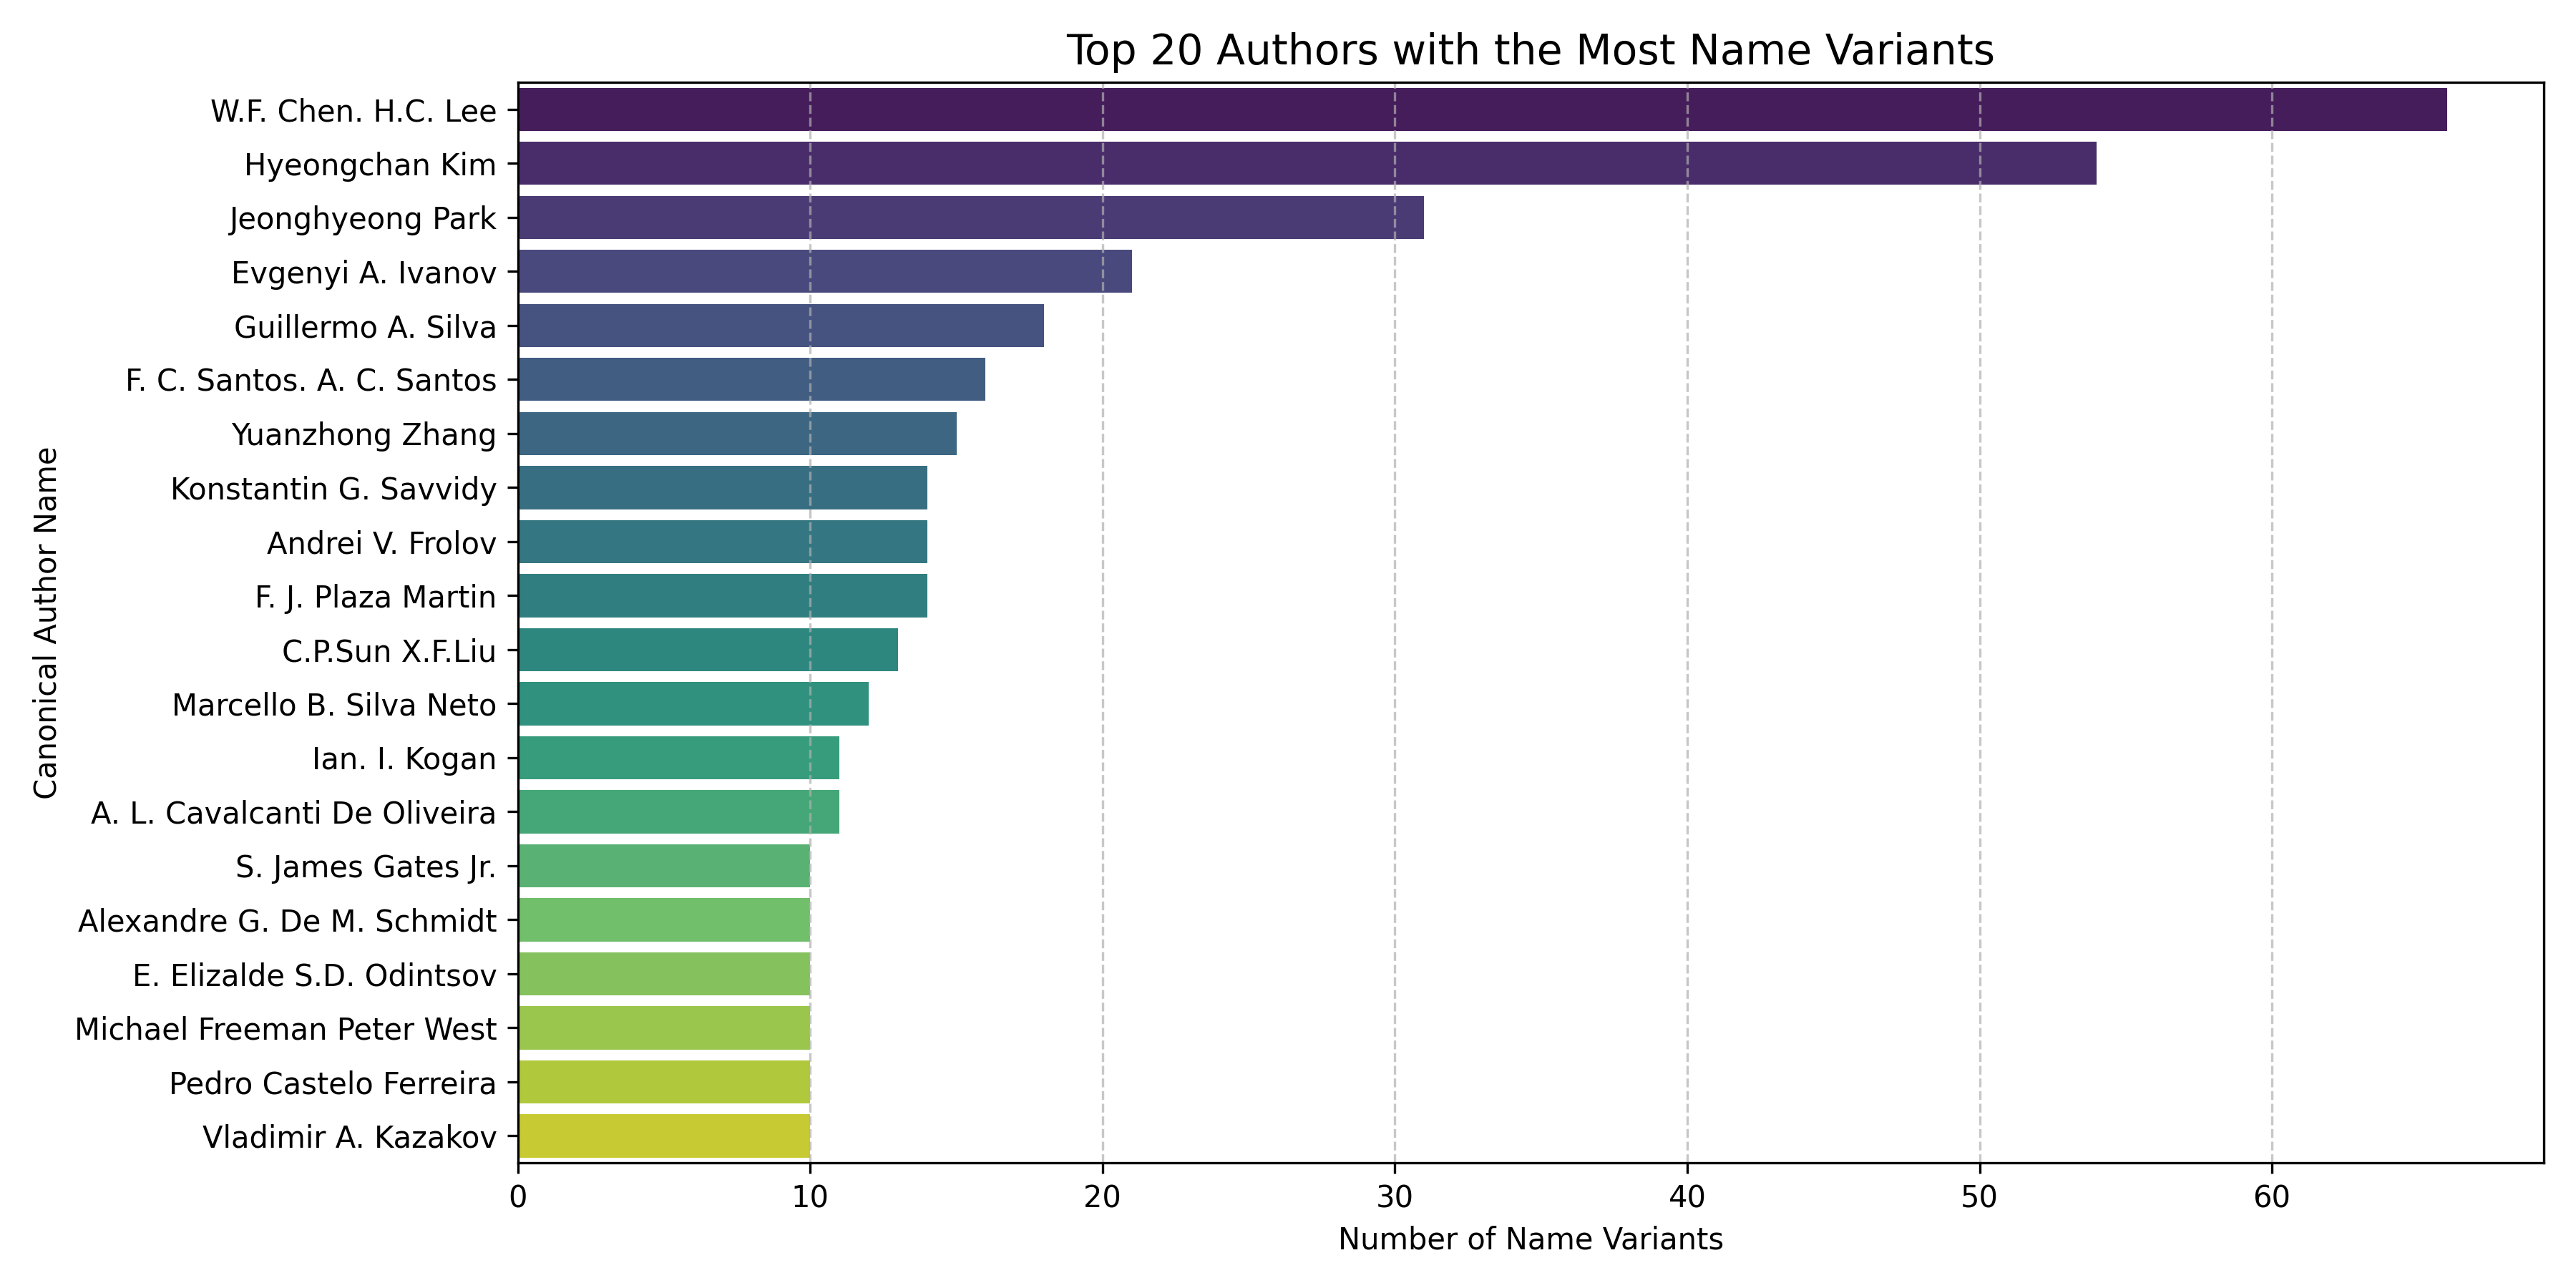
\includegraphics[width=0.95\textwidth]{pictures/top_author_name_variants.png}
    \caption{Top 20 authors with the most name variants in the dataset.}
    \label{fig:name_variants_bar}
\end{figure}

As shown in Figure~\ref{fig:name_variants_bar}, some prolific authors appear under 6 or more name forms. This is especially common for:
\begin{itemize}
    \item Authors with long names or multiple initials
    \item Names of non-Western origin that are variably formatted
    \item Authors active during the early arXiv years, when naming conventions were less standardized
\end{itemize}

This visualization illustrates the necessity of a robust normalization pipeline. Without resolving these variants, collaboration and citation networks would misrepresent the underlying author structure, inflating node counts and distorting community detection outcomes.



\subsection{Quantitative Summary}

The name normalization pipeline produced the following statistics:
\begin{itemize}
    \item \textbf{Initial raw names:} 14420
    \item \textbf{Unique cleaned names:} 14605
    \item \textbf{Final standardized names:} 8344
    \item \textbf{Average variants per standard name:} 1.75
\end{itemize}

\begin{figure}[H]
    \centering
    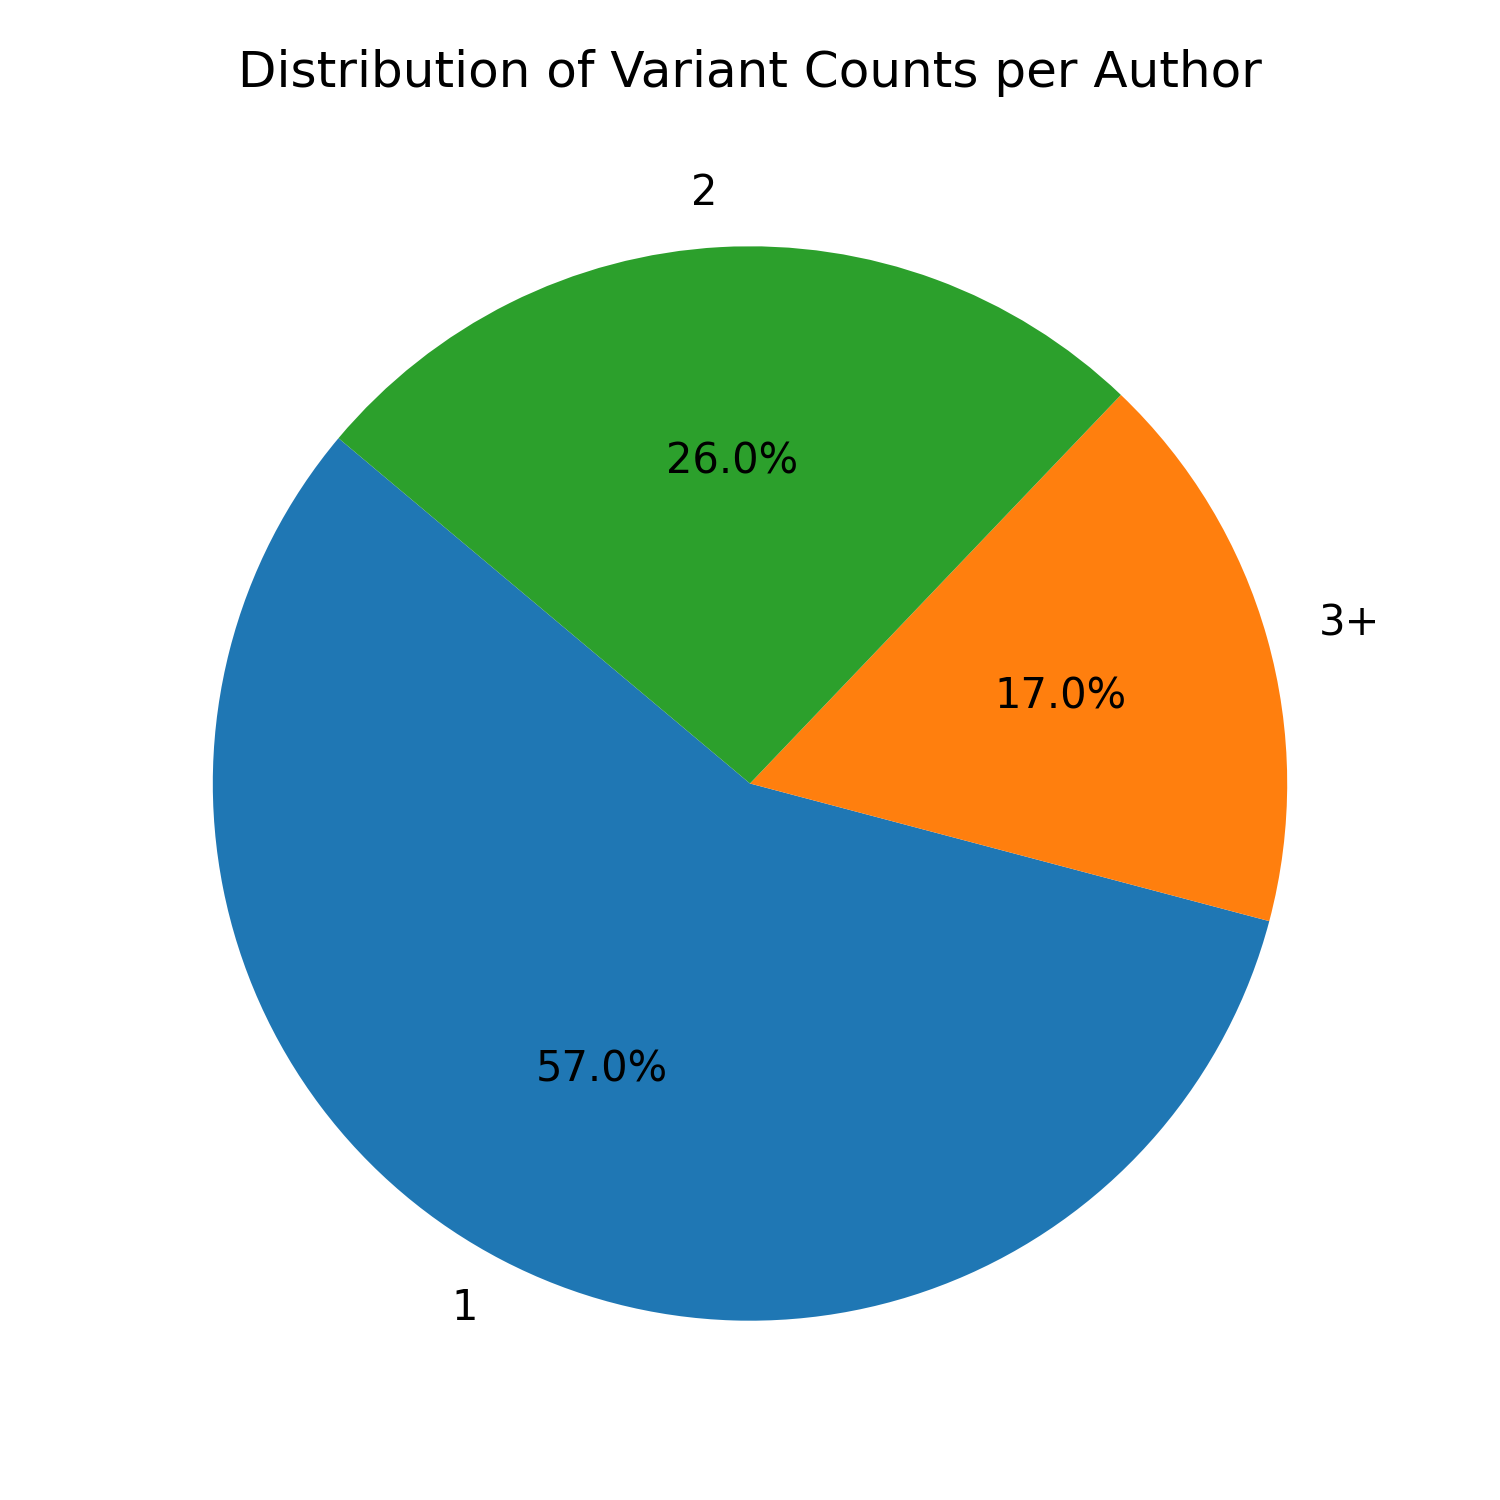
\includegraphics[width=0.45\textwidth]{pictures/variant_distribution_pie.png}
    \caption{Proportion of authors with 1, 2, or more name variants.}
\end{figure}


\subsection{Challenges and Limitations}

Despite a robust pipeline, several edge cases remain difficult:
\begin{itemize}
    \item Ambiguous abbreviations that match multiple possible full names
    \item Authors with common surnames (e.g., ``Zhang'') and sparse first-name information
    \item Homonyms (distinct individuals with identical names)
\end{itemize}

Future improvements could include:
\begin{itemize}
    \item Cross-referencing external author databases (e.g., ORCID, DBLP)
    \item Including affiliation or co-author context to disambiguate
\end{itemize}

\subsection{Polished file}

Finally, we use \texttt{convert.py} to integrate our results from \texttt{author\_variants.json} and \texttt{output.json} to create \texttt{papers\_standardized.json}, which is clean enough for future usage.

This script performs a key standardization step: it maps all detected author name variants back to a canonical author identifier, ensuring consistency in authorship across papers. For each paper, it replaces original author names with their standardized forms and retains the full metadata. The resulting \texttt{papers\_standardized.json} file contains a list of processed papers, each with uniform author attributions and previously extracted metadata (e.g., title, abstract, keywords, citation links).

This clean format facilitates downstream tasks such as building citation graphs, clustering papers by topic, and performing bibliometric analysis.

\section{Graph Construction and Community Detection}

To explore the collaborative structure of the scientific community in theoretical physics, we construct a graph where each node corresponds to an author and each edge represents a co-authorship relationship. This abstraction provides a powerful framework to analyze collaboration patterns, community structure, and network centrality. This part can be found in \texttt{physics.ipynb}.

We use a following steps to begin our work:
1. construct a graph based on the relation of collabration where the nodes are the authors and with egde weighted by the times of collabration.
2. we calculate the community of this graph.
3. we create a new graph with i) each node is a community, ii) the edge is weighted by the net citation between groups.4.We visualize the graph of communities.

\subsection{Construction of the Author Collaboration Graph}

The author collaboration network is modeled as an undirected, weighted graph $G = (V, E, w)$, where:

\begin{itemize}
    \item $V$ is the set of nodes, each representing a unique author.
    \item $E$ is the set of undirected edges $(u, v)$ such that authors $u$ and $v$ have co-authored at least one paper.
    \item $w: E \rightarrow \mathbb{N}$ is a weight function where $w(u,v)$ denotes the number of papers jointly authored by $u$ and $v$.
\end{itemize}

The dataset used to build this graph is the CA-HepTh collaboration network from arXiv, which consists of metadata of physics papers in the High-Energy Theory category. For each paper, the list of authors is parsed, and all pairwise combinations are formed using $\binom{n}{2}$ for a paper with $n$ authors. Each pair contributes an edge in the graph, with repeated collaborations incrementing the corresponding edge weight.

\vspace{0.3cm}
\textbf{Implementation.} The graph is implemented using the \texttt{NetworkX} Python library. Nodes are assigned integer IDs corresponding to cleaned author names, and edges are stored in an adjacency list for efficient processing.

\subsubsection*{Graph Statistics}

After preprocessing, the graph contains:
\begin{itemize}
    \item \textbf{8187 nodes} (unique authors)
    \item \textbf{19205 edges} (co-authorship relationships)
    \item An average node degree of approximately \textbf{4.69}
\end{itemize}

The network exhibits a heavy-tailed degree distribution, indicating the presence of a few highly collaborative authors alongside a majority with limited connections. Most authors are part of a single giant component, illustrating the interconnected nature of the theoretical physics community.

\vspace{0.3cm}
\textbf{Interpretation.} This co-authorship graph encodes rich structural information about the scientific community. Local neighborhoods of nodes often correspond to research groups or subfields, while global topology reveals patterns of interdisciplinary collaboration and academic influence. By studying the graph structure, we can:
\begin{itemize}
    \item Identify tightly-knit research groups (communities)
    \item Examine the centrality and influence of individual authors
    \item Quantify collaboration density across subdomains
\end{itemize}

\vspace{0.3cm}
Figure~\ref{fig:collab} provides a visualization of a sample subgraph with authors colored by detected community.

\begin{figure}[H]
    \centering
    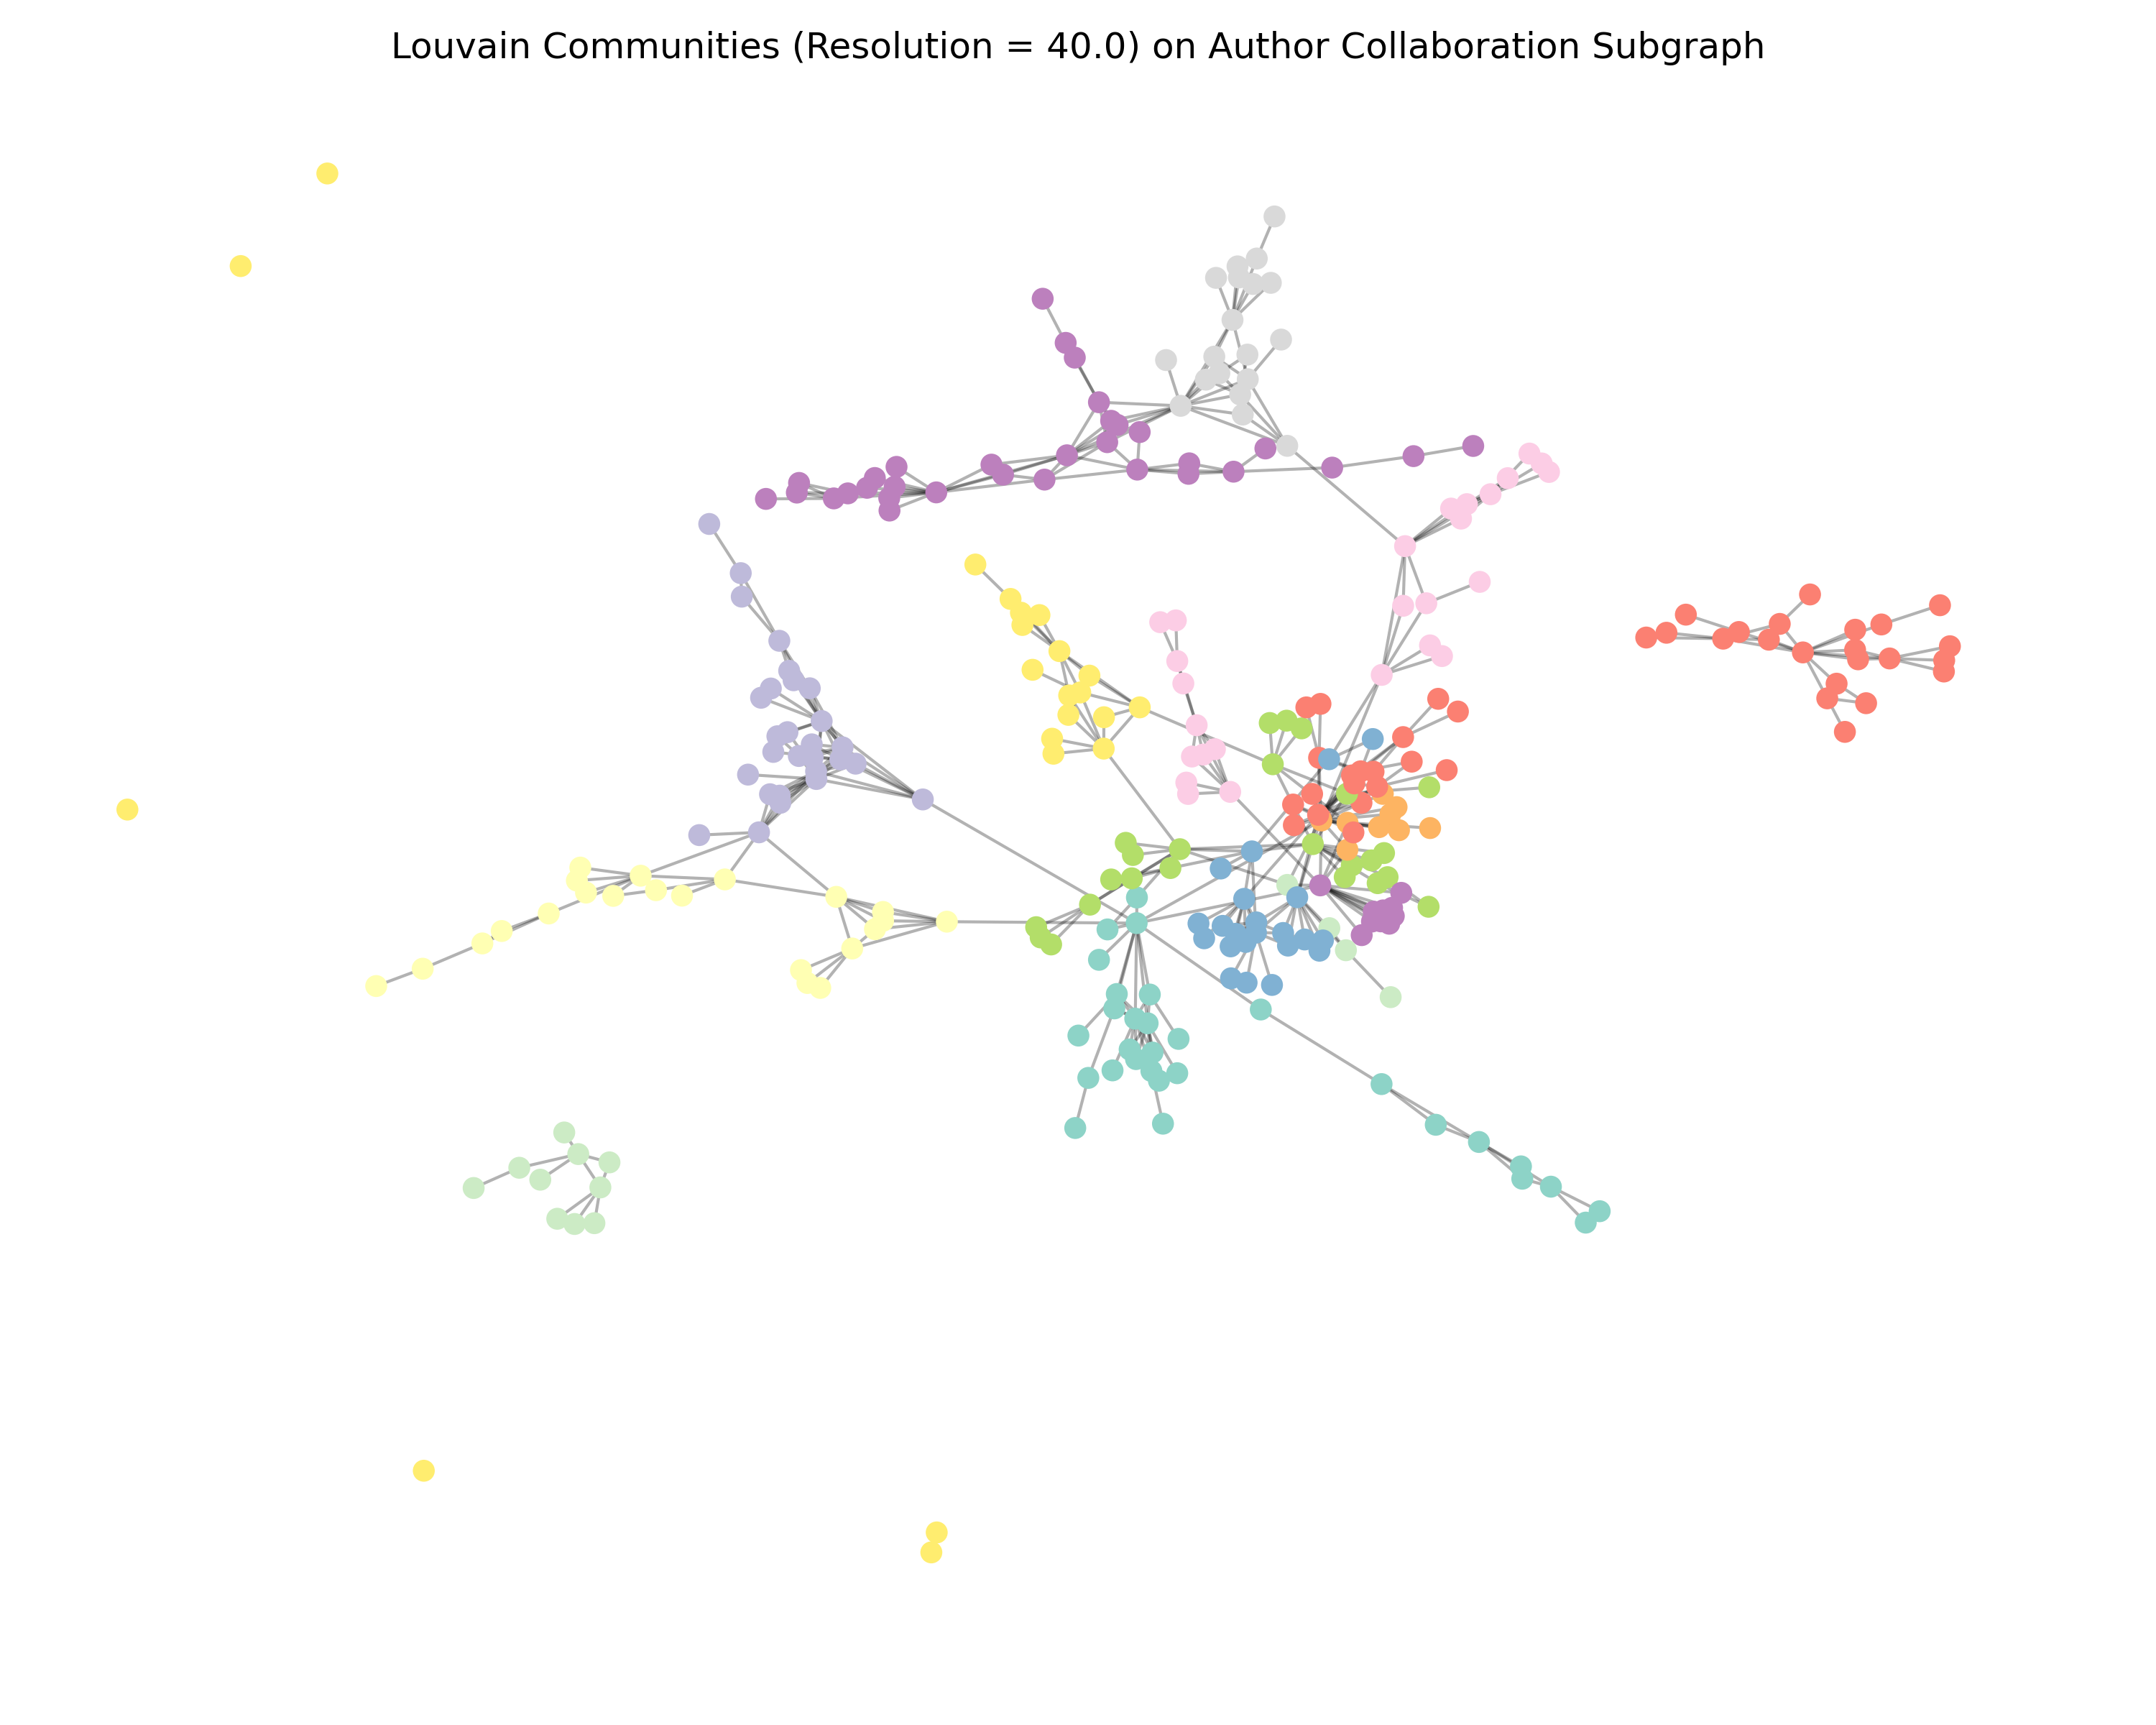
\includegraphics[width=0.8\textwidth]{pictures/collab_graph_louvain_sample.png}
    \caption{Sample visualization of author collaboration network with Louvain community detection. Nodes are authors; edges represent co-authorships; colors denote communities.}
    \label{fig:collab}
\end{figure}

\subsection{Community Detection Methods}

To uncover the latent structure of the collaboration graph, we apply three community detection algorithms. These algorithms identify clusters of authors who collaborate more frequently with each other than with the rest of the network. Each method has distinct theoretical foundations and computational properties.

\subsubsection*{1. Louvain Method (Modularity Optimization)}

The Louvain method is a greedy optimization algorithm that attempts to maximize the modularity score of a partition. Modularity measures the density of links inside communities compared to links between communities. The algorithm operates in two phases:
\begin{itemize}
    \item Initially, each node is assigned to its own community. The algorithm iteratively merges neighboring communities if doing so increases the overall modularity.
    \item Once no further improvement is possible, a new graph is constructed where each community becomes a node, and the process is repeated recursively.
\end{itemize}

This method is computationally efficient and widely used for large networks. In our graph, the Louvain method detected \textbf{1542 communities}.

\subsubsection*{2. Clique Percolation Method (CPM)}

The Clique Percolation Method identifies communities as chains of adjacent $k$-cliques — complete subgraphs of $k$ nodes — that share $k-1$ nodes. Unlike modularity-based methods, CPM allows for overlapping communities, which is particularly relevant in social networks where individuals may belong to multiple groups.

For our implementation, we used a 3-clique percolation. This approach captured \textbf{1161 overlapping communities}, emphasizing tightly-bound collaborative subgroups within the larger research community.

\subsubsection*{3. Label Propagation Algorithm (LPA)}

Label Propagation is an iterative and parameter-free algorithm that initializes each node with a unique label. At each iteration, a node adopts the most frequent label among its neighbors. The process continues until convergence, resulting in dense communities where nodes share the same label.

This method is extremely fast and suitable for large graphs. Its simplicity, however, may lead to instability or resolution limits. In our experiment, the algorithm identified \textbf{1994 communities}.

\subsubsection*{Comparison and Insights}

Each algorithm provides a different perspective on the graph’s structure:
\begin{itemize}
    \item Louvain detects communities optimized for modularity, often yielding interpretable and balanced partitions.
    \item Clique Percolation captures fine-grained, overlapping collaboration groups.
    \item Label Propagation uncovers a broad range of communities efficiently, though results can vary due to random initialization.
\end{itemize}

The variation in the number of communities reflects the nature of each algorithm’s assumptions and resolution. Figure~\ref{fig:collab} illustrates an example where communities detected by Louvain are visualized through node coloring.

\subsection{Graph of Communities}

To understand how collaborative groups interact on a broader scale, we construct a higher-level graph where each node corresponds to a community previously identified using the Louvain algorithm. This abstraction allows us to study inter-community dynamics and structural patterns beyond individual collaborations.

\subsubsection*{Definition and Construction}

We define the \textbf{community graph} $G_c = (V_c, E_c)$ as follows:
\begin{itemize}
    \item Each node in $V_c$ represents a community discovered in the author collaboration graph using the Louvain method with resolution $= 40.0$.
    \item An undirected edge $(C_i, C_j) \in E_c$ is added if at least one co-authorship link exists between any author in community $C_i$ and any author in community $C_j$.
    \item The weight of each edge corresponds to the number of such inter-community links.
\end{itemize}

This transformation captures how collaborative groups (not just individuals) are interlinked and can reveal mesoscale organizational patterns in the scientific network.

\subsubsection*{Graph Statistics}

After constructing the community-level graph, we obtain the following summary:

\begin{itemize}
    \item \textbf{Number of nodes:} 1542 communities
    \item \textbf{Number of edges:} 13053 inter-community connections
    \item \textbf{Average degree:} $\langle k \rangle \approx 16.93$
    \item The graph is sparse but highly connected, indicating broad interactions across research communities.
\end{itemize}

\subsubsection*{Structural Interpretation}

The community graph provides a complementary view to the author graph:
\begin{itemize}
    \item Densely connected regions may correspond to interdisciplinary subfields or long-standing collaborations between major groups.
    \item Sparse or peripheral communities might represent isolated or niche research topics.
    \item Communities that serve as bridges between otherwise disconnected modules could be of particular importance for knowledge dissemination.
\end{itemize}

\begin{figure}[H]
    \centering
    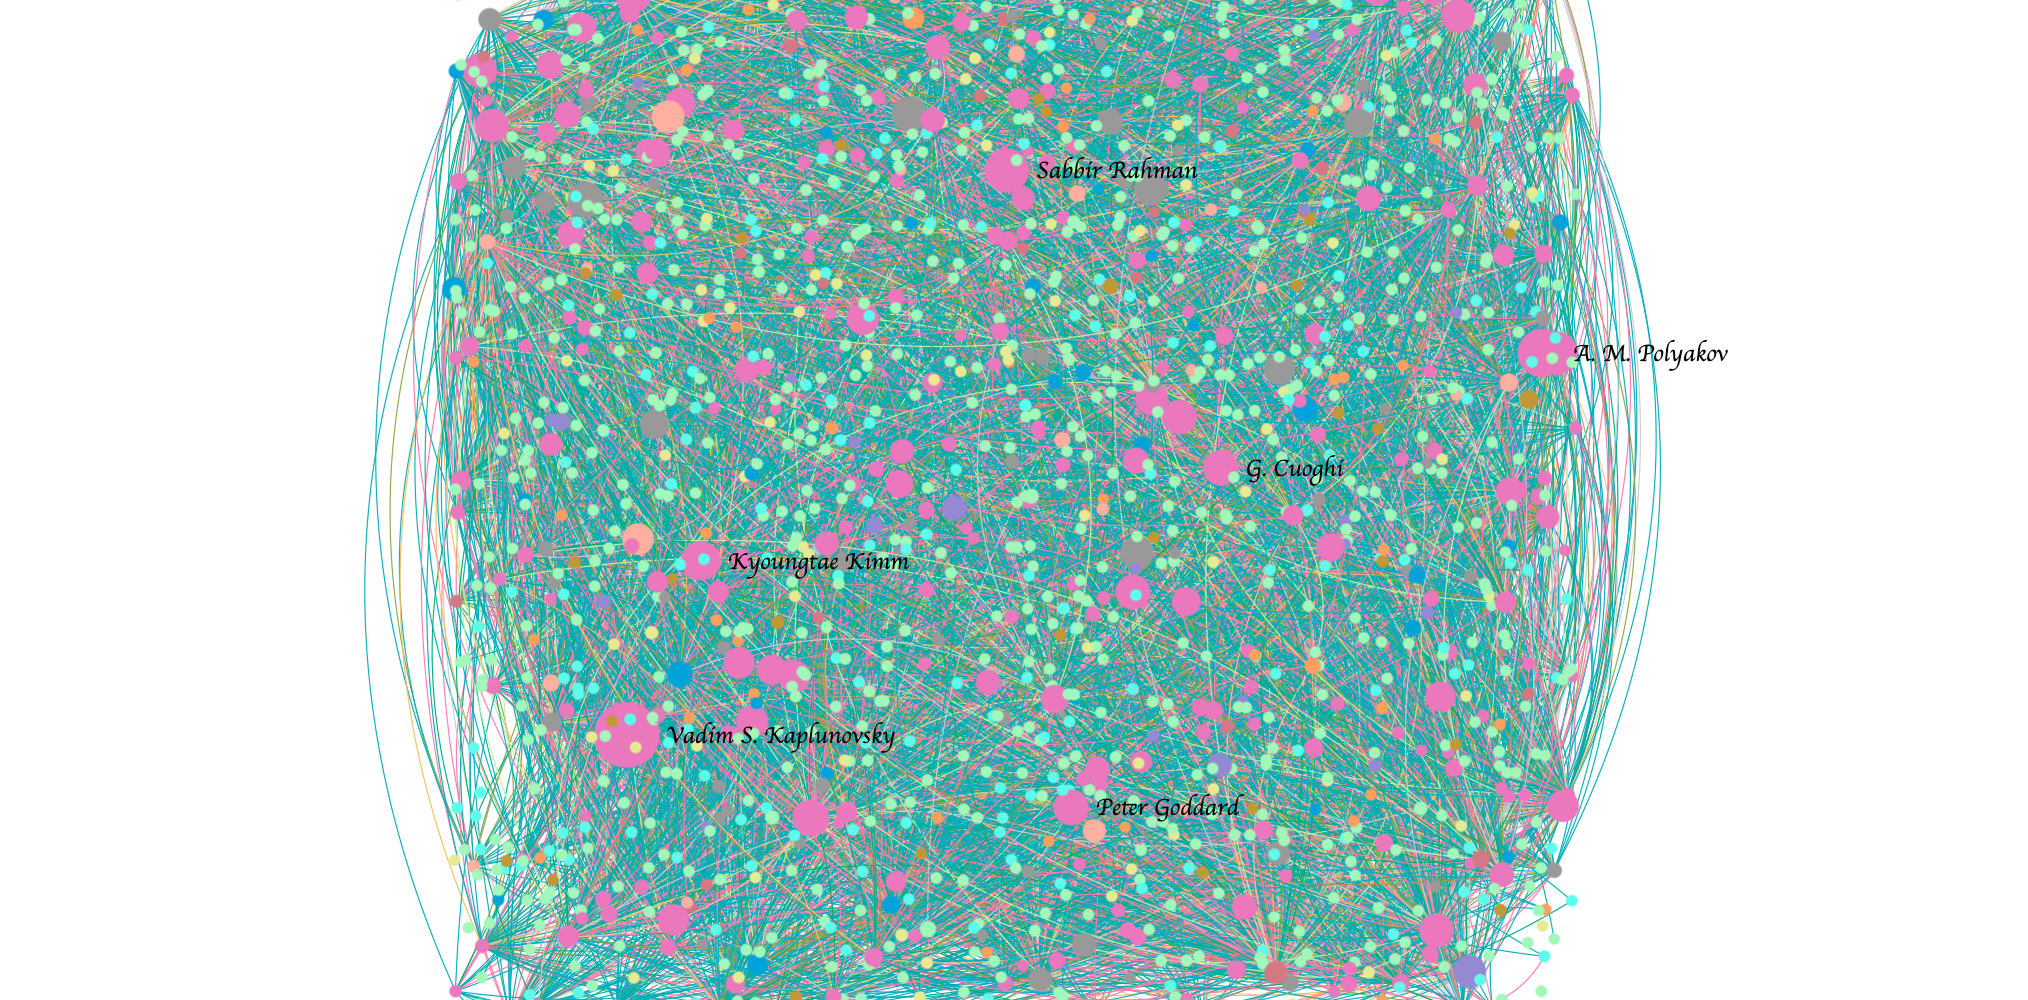
\includegraphics[width=0.95\textwidth]{pictures/graph-2.png}
    \caption{Graph of communities: nodes represent Louvain-detected communities, edges indicate collaborative links across communities.}
\end{figure}

\begin{figure}[H]
    \centering
    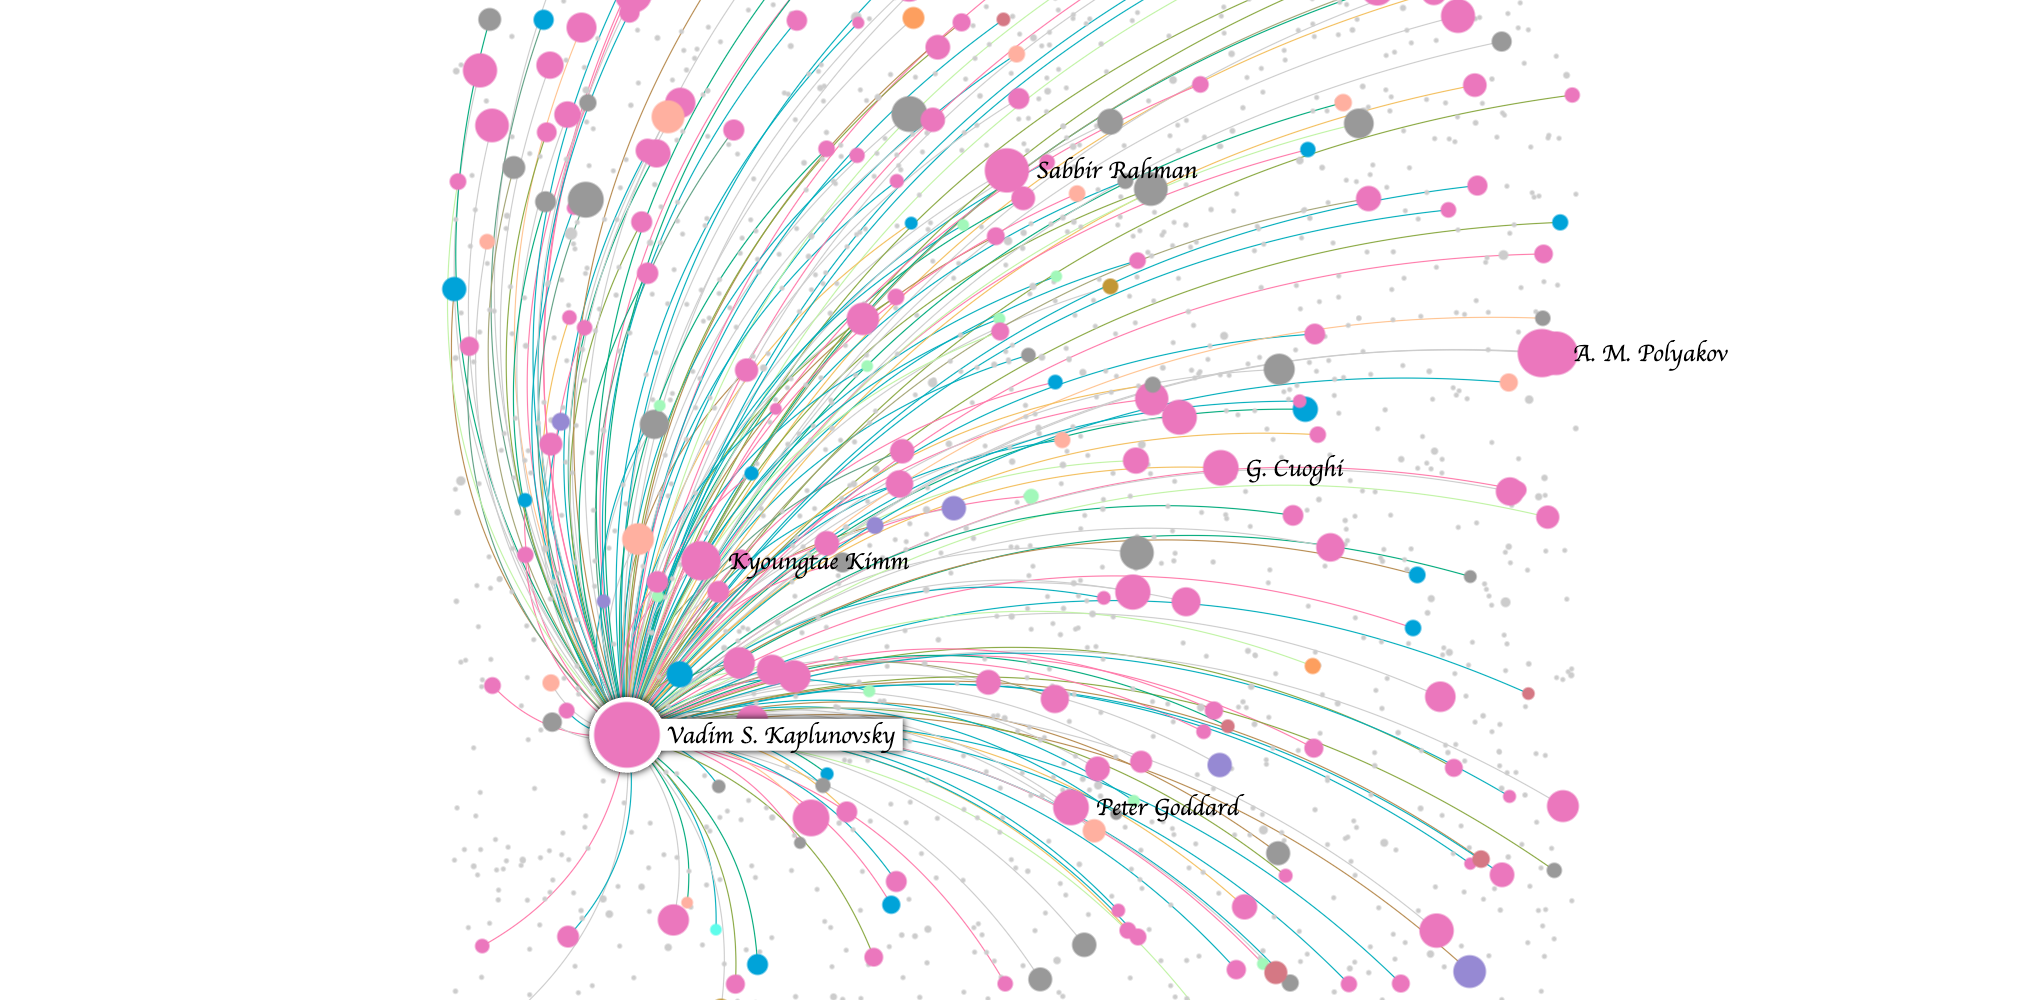
\includegraphics[width=0.95\textwidth]{pictures/graph2-2.png}
    \caption{A large commnunity example}
\end{figure}




\section{Keywords analysis}

To further enrich our understanding of the collaboration network, we analyze the keywords associated with each paper. Keywords provide insights into the topical focus of research and can help identify trends, emerging areas, and shifts in scientific discourse over time.

\subsection{Keyword Extraction and BertKey}

To extract meaningful semantic keywords from the abstracts, we adopt \texttt{BertKey}, a keyword extraction method based on transformer models. Unlike traditional statistical methods such as TF-IDF or TextRank, \texttt{BertKey} uses contextual embeddings from pretrained BERT models to capture the semantic importance of tokens within each document.

Our implementation, provided in the script \texttt{mot.py}, proceeds as follows. First, each abstract is tokenized and passed through a pretrained BERT model to obtain contextualized embeddings for every token. Then, we compute the average embedding of the entire sentence as a representation of the overall context. Each token’s importance score is estimated by measuring its cosine similarity with the sentence embedding. Tokens with the highest scores are selected as keywords.

To avoid selecting non-informative tokens such as punctuation or stopwords, we apply additional filtering heuristics and only retain meaningful subword tokens. For each abstract, the top three ranked keywords are extracted and saved to a JSON file. These extracted keywords form the basis for subsequent domain clustering and visualization tasks.

We also note that the extraction process is computationally intensive. On the computer with GPU NVIDIA GeForce RTX 3090, and it takes usually 3 hours to extract all keywords from 29555 abstracts.

\subsection{Keyword Integration}

After extracting keywords for each paper using \texttt{BertKey}, we integrate them into the main dataset by matching paper identifiers. This step ensures that the semantic keywords are directly associated with the corresponding metadata such as titles, abstracts, authors, and timestamps.

\subsubsection*{Techniques and Input/Output Description}

The core keyword extraction pipeline relies on several key components:

\begin{itemize}
  \item \textbf{Transformer-based embeddings:} We use the \texttt{bert-base-uncased} model from HuggingFace's Transformers library to generate contextual token embeddings. This allows each word’s representation to reflect its meaning in context.
  
  \item \textbf{Cosine similarity scoring:} Each token embedding is compared with the mean sentence embedding using cosine similarity. This quantifies how semantically central a token is to the overall meaning of the abstract.

  \item \textbf{Heuristic post-filtering:} Special tokens like \texttt{[CLS]}, subword fragments, and low-content tokens are filtered out to retain only meaningful keywords.
  
  \item \textbf{Top-K selection:} After ranking all valid tokens, the top 3 keywords are selected for each paper.
\end{itemize}

The script \texttt{mot.py} takes as input a JSON file containing paper abstracts. Each entry must contain a unique paper ID and its corresponding abstract. The output is another JSON file where each paper ID is associated with a list of three extracted keywords. This file serves as the keyword metadata for further processing.

Additionally, the script \texttt{merge-keywords.py} is used to combine and standardize multiple keyword outputs (e.g., variants or different versions). It reads intermediate files such as \texttt{bertkey.json} and \texttt{author\_variants.json}, and produces a merged result in a unified format, typically named \texttt{keywords\_cleaned.json}.


To ensure consistency, entries without matching keywords are either discarded or kept without the keyword field, depending on configuration. This integrated dataset serves as the input for downstream clustering, visualization, and analysis tasks.

\section{Visualisation et Analyse du Réseau de Citations de la Physique Théorique}

Ce notebook a pour objectif de construire et visualiser un graphe de citations entre des articles scientifiques issus du domaine de la physique théorique à partir du corpus ArXiv (catégorie High Energy Physics - Theory, ``Cit-HepTh''). Il combine traitement de texte, nettoyage sémantique, clustering non supervisé, et visualisation temporelle.

\subsection{Prétraitement des mots-clés}

Deux fichiers sont d'abord intégrés :
\begin{itemize}
    \item \texttt{keywords\_extracted.jsonl} : chaque ligne contient les mots-clés extraits automatiquement d'un article donné.
    \item \texttt{keyword\_clusters.json} : il contient des regroupements de synonymes (par exemple, ``vortex filament'' et ``vortex gas'' sont normalisés en ``vortex cells'').
\end{itemize}

Un script de nettoyage applique cette normalisation pour chaque mot-clé, produisant un dictionnaire final \texttt{keywords\_cleaned.json} qui associe à chaque article un ensemble de mots-clés uniques et normalisés.

\subsection{Construction du graphe de citations}

À partir du fichier brut \texttt{Cit-HepTh.txt}, un graphe orienté est construit via la librairie \texttt{networkx}. Chaque nœud représente un article, et chaque arête représente une relation de citation. Les métadonnées (titre, mots-clés nettoyés) sont intégrées aux nœuds.

\subsection{Détection de communautés et classification thématique}

Deux stratégies complémentaires sont utilisées :
\begin{itemize}
    \item Détection de communautés via l'algorithme de Louvain, révélant des sous-structures denses dans le graphe.
    \item Classification thématique supervisée par clustering KMeans sur les représentations TF-IDF des mots-clés, assignant un domaine scientifique à chaque article. Chaque domaine reçoit une couleur distincte.
\end{itemize}

\begin{figure}[H]
    \centering
    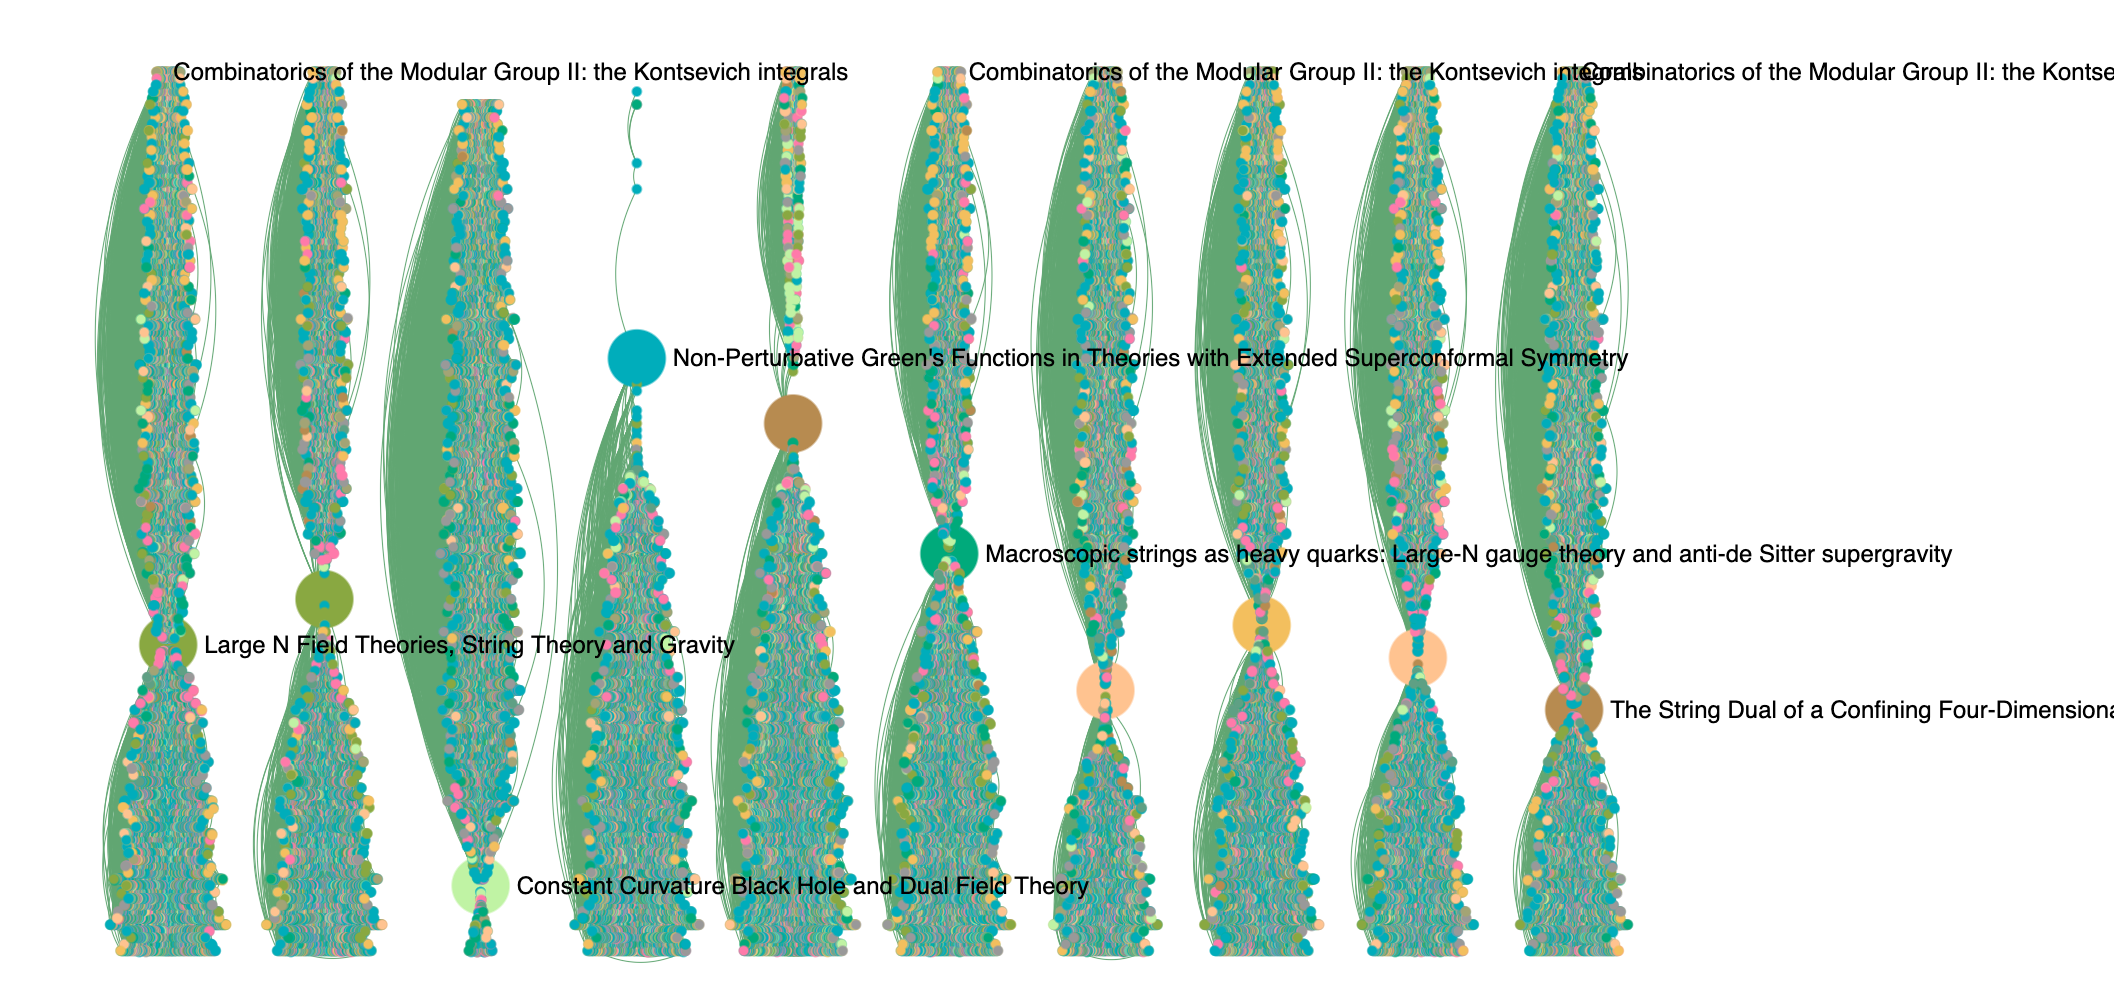
\includegraphics[width=0.95\textwidth]{pictures/graph.png}
    \caption{Visualisation globale du graphe des citations, où la taille des nœuds reflète leur centralité d’intermédiarité (betweenness centrality).}
\end{figure}

\subsection{Projection temporelle et positionnement}

Les articles sont positionnés dans l'espace en deux dimensions :
\begin{itemize}
    \item Axe horizontal : domaines scientifiques (issus du clustering KMeans sur les mots-clés);
    \item Axe vertical : date de soumission de l’article (extrait de l’identifiant ArXiv).
\end{itemize}

Des offsets latéraux sont ajoutés pour éviter le chevauchement. La taille des nœuds reflète leur degré (nombre de citations reçues ou faites).

\begin{figure}[H]
    \centering
    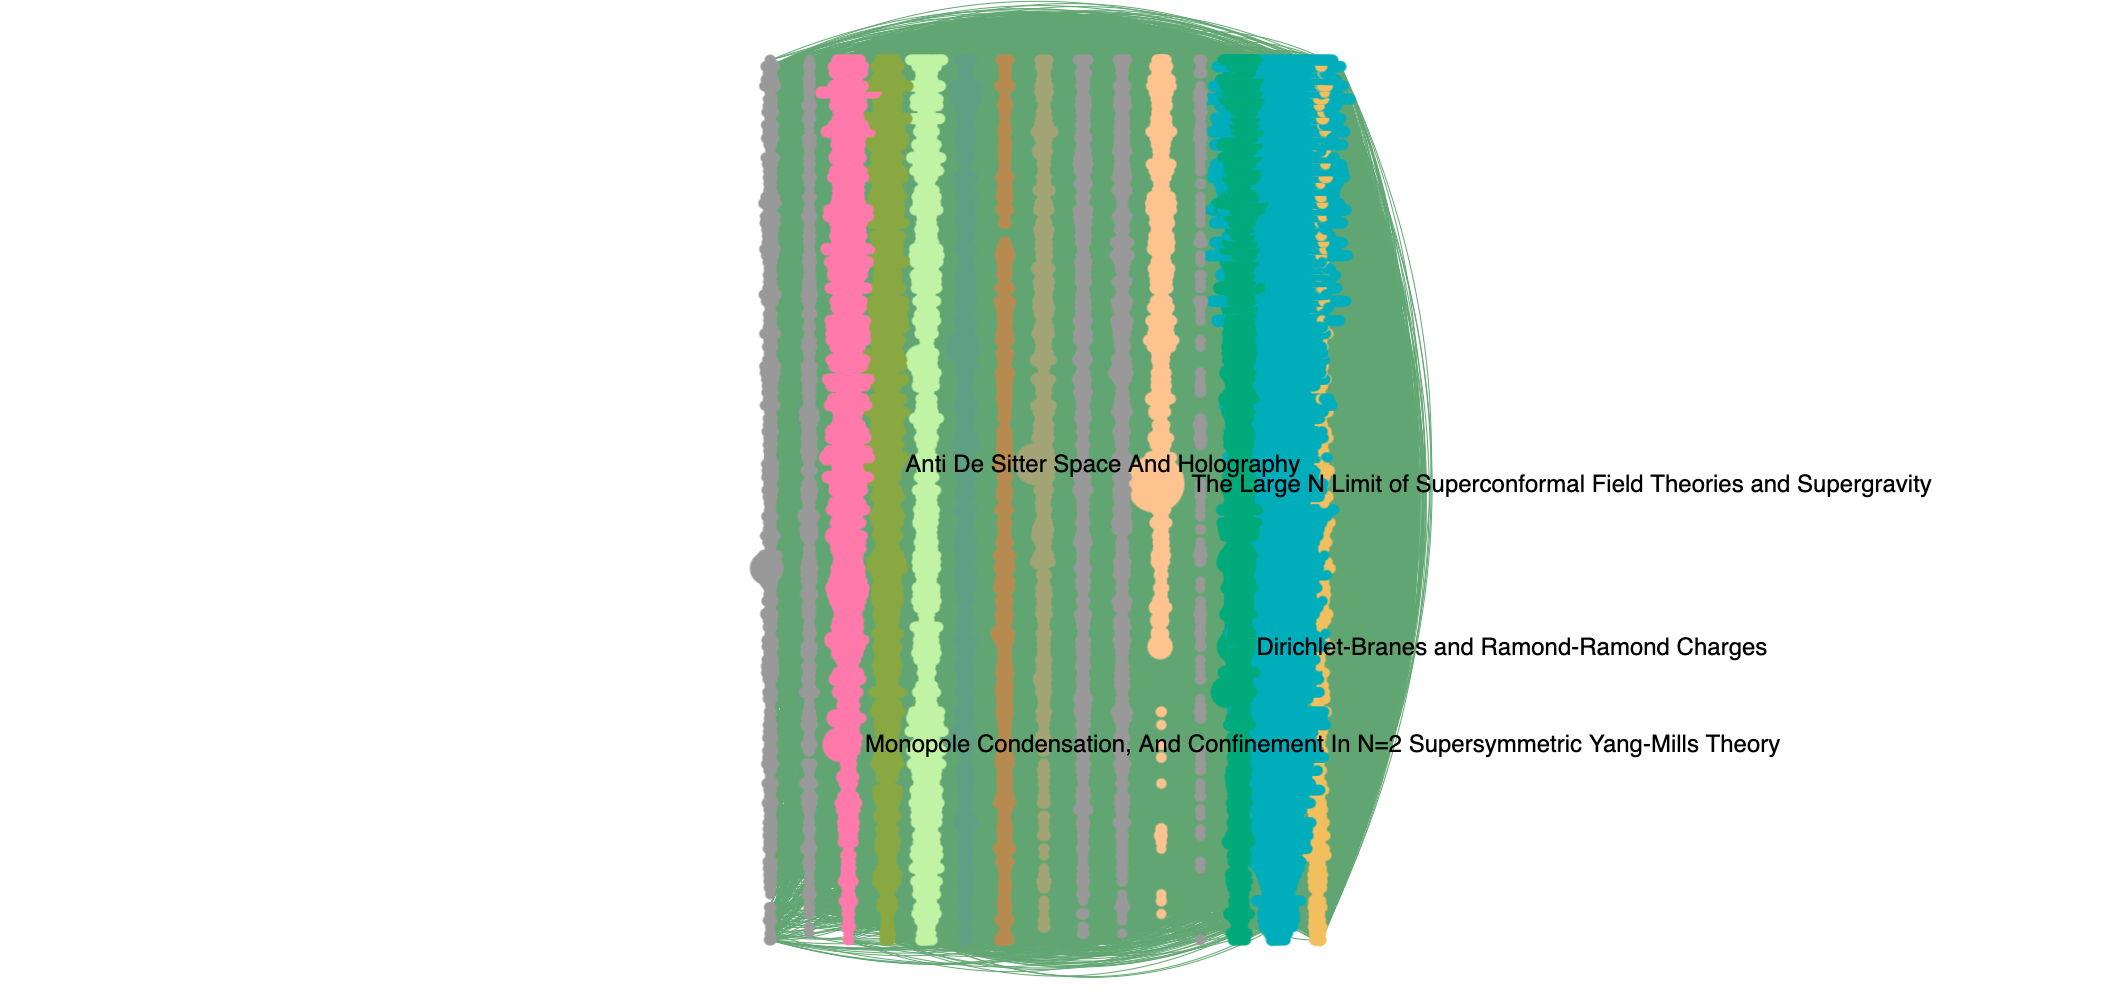
\includegraphics[width=0.95\textwidth]{pictures/domain.png}
    \caption{Projection temporelle et thématique des articles. Chaque colonne correspond à un domaine scientifique identifié automatiquement, les couleurs représentant les communautés détectées.}
\end{figure}

\subsection{Exploration temporelle structurée des trajectoires de citations}

Une fois les articles classés et placés dans l’espace, une analyse plus fine est réalisée sur les \textbf{10 articles les plus centraux}, mesurés par leur \textit{betweenness centrality}.

Pour chacun de ces articles, on construit deux sous-arbres temporels :
\begin{itemize}
    \item Un arbre descendant (\textit{forward direction}) : les articles que cet article cite, avec propagation récursive vers leurs propres citations.
    \item Un arbre ascendant (\textit{backward direction}) : les articles qui citent cet article, avec propagation récursive vers leurs propres référents.
\end{itemize}

Chaque nœud dans ces sous-arbres est une \textbf{copie} d’un article original, étiqueté par son origine (par ex. \texttt{9211012\_from\_9802150}) pour éviter les conflits d’identifiants et garantir un graphe acyclique. La profondeur temporelle est limitée à une fenêtre de $N=120$ mois pour éviter les branches trop longues.

La position verticale des nœuds dans l’arbre est centrée autour de la date du nœud racine (les $10$ top articles), permettant une visualisation comparative claire entre branches ascendantes et descendantes. L’arborescence complète est ainsi structurée par origine thématique et temporelle.

\begin{itemize}
    \item Les arêtes sont orientées (ascendantes ou descendantes).
    \item La taille des nœuds est proportionnelle à leur importance locale (degré).
    \item Les couleurs reflètent les domaines thématiques (KMeans).
\end{itemize}

Cette approche permet de visualiser des dynamiques telles que :
\begin{itemize}
    \item L'impact durable d’un article dans un champ ;
    \item Les échos successifs d’un article dans la littérature scientifique ;
    \item L’évolution thématique d’une lignée de travaux.
\end{itemize}

\section{Future Work}
\begin{itemize}
\item Expand to full arXiv corpus
\item Integrate institutional metadata
\item Develop interactive graph dashboards
\item Apply GNNs to predict future collaborations
\end{itemize}

\section{Conclusion}
Project CURA demonstrates the value of graph-based data mining in understanding scientific collaboration. Our work offers a blueprint for replicable analysis across domains and sets the stage for dynamic, real-time monitoring of research networks.

\newpage

\section*{Appendix}
\subsection*{A. Tools and Libraries}
\begin{itemize}
\item Python 3.11
\item NetworkX
\item matplotlib, seaborn
\item community (Louvain)
\item pandas, numpy
\item BertKey (HuggingFace Transformers)
\item scikit-learn (KMeans)
\item PyTorch (for BertKey)
\item regex (for text processing)
\item json (for data serialization)
\item tqdm (for progress bars)
\item nltk (for text normalization)
\end{itemize}

\subsection*{B. Scripts and Notebooks}
\begin{itemize}
\item \texttt{First\_Extraction.py} - initial metadata extraction
\item \texttt{convert.py} - transforms dataset into graph format
\item \texttt{nom.py} - author name preprocessing
\item \texttt{standarniee\_name.py} - alias mapping
\item \texttt{physics.ipynb} - analysis and plotting
\item \texttt{mot.py} - keyword extraction with BertKey
\item \texttt{merge-keywords.py} - keyword normalization
\item \texttt{graph\_visualization.ipynb} - interactive graph exploration
\item \texttt{graph\_citation.ipynb} - citation graph analysis
\end{itemize}


\end{document}

